\documentclass[10pt]{beamer}
\usepackage{datetime}

% \usepackage{fontspec}
% \setmainfont[Path = fonts/,
%     UprightFont = *-Regular,
%     ItalicFont = *-Italic
%  ]
% {FiraSans}
\usetheme[progressbar=frametitle, everytitleformat=uppercase,
plaintitleformat=uppercase, block=transparent]{m}

\usepackage{booktabs}
\usepackage[scale=2]{ccicons}
\usepackage{adjustbox}
\usepackage[backend=biber]{biblatex}

\usepackage{pgfplots}
\usepgfplotslibrary{dateplot}
\usetikzlibrary{shapes,automata,positioning,arrows,calc}
\usepackage{pgfplots,wrapfig}

\definecolor{bg}{HTML}{F4F4EE}
% E8E8E3
\definecolor{bg_d}{HTML}{E8E8E3}
\definecolor{bg_dd}{HTML}{D4D4CE}
\definecolor{primary}{HTML}{607D8B}
\definecolor{primary_dark}{HTML}{455A64}
\definecolor{secondary}{HTML}{FF5722}

\usepackage{xcolor}
\colorlet{blocktitlebgcolor}{bg}
\colorlet{blocktitlefgcolor}{primary_dark}
\colorlet{titlebgcolor}{primary}
\colorlet{accentcolor}{secondary}
\colorlet{blockbodybgcolor}{white}
\colorlet{blockbodyfgcolor}{primary_dark}
\colorlet{backgroundcolor}{bg}

\usepackage{array}
\usepackage{varwidth}

\setbeamercolor{progressbar}{fg=accentcolor, bg=accentcolor!40!black}
% \usepackage{tabularx}
% \usepackage{pgfpages}
% \setbeameroption{show notes}
% \setbeameroption{show notes on second screen}

% \usemintedstyle{trac}

% \setbeamercolor{normal text}{fg=white, bg=black}
% \setbeamercolor{alerted text}{fg=green, bg=black}
\colorlet{mDarkTeal}{primary}
% \definecolor{mLightBrown}{HTML}{F7E300}
% \definecolor{mDarkBrown}{HTML}{A69B29}
% \definecolor{mLightGreen}{HTML}{F7E300}

% \definecolor{mLightGolden}{HTML}{F7E300}
% \definecolor{mDarkGolden}{HTML}{A69B29}

% \setbeamercolor{progress bar}{fg=mLightGolden, bg=mDarkGolden}

\title{DSaaS}
\subtitle{A Cloud Service for Persistent Data Structures}
\newdate{date}{24}{04}{2016}
\date{\displaydate{date}}
\author{Pierre le Roux, Steve Kroon and Willem Bester}
\institute{Stellenbosch University \\ \url{http://cs.sun.ac.za/~kroon/dsaas}}

\begin{document}

\newcommand{\architectureOverview}[0]{
    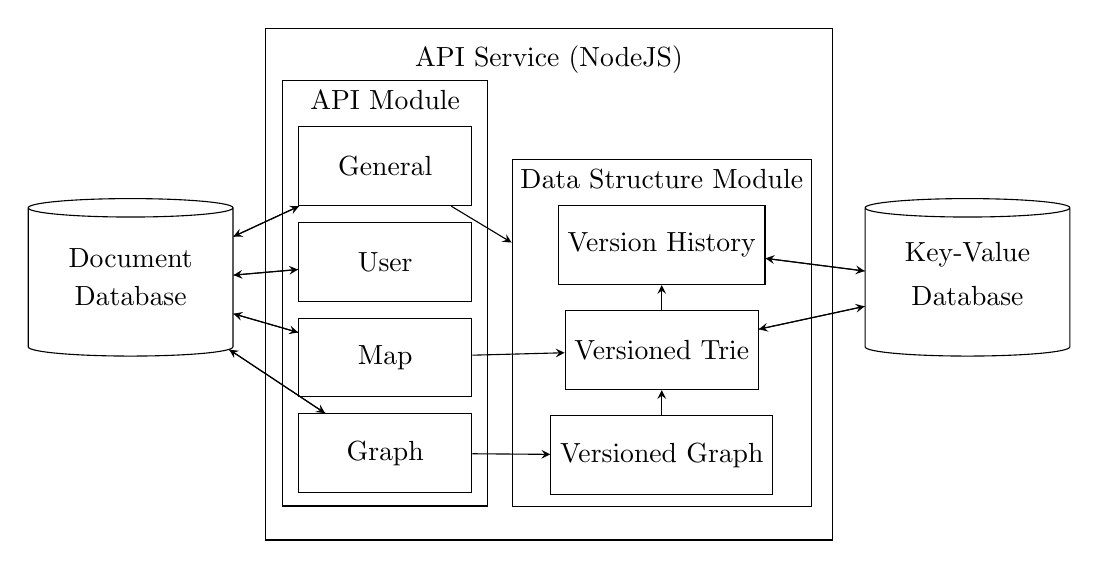
\begin{tikzpicture}

    \tikzstyle{obj}=[draw, rectangle, minimum height=1cm, minimum width=2.2cm];
    \tikzstyle{bigobj}=[draw, rectangle, minimum height=2.5cm, minimum width=3.5cm];
    \tikzstyle{db}=[cylinder, shape border rotate=90, draw,minimum height=2cm,minimum width=2.6cm];

    \begin{scope}[>=stealth]
      \node (serverContainer) at (0,0) [draw, rectangle, minimum height=6.5cm, minimum width=7.2cm]{};
      \node [above=-0.7cm of serverContainer]{API Service (NodeJS)};

      \node (db1) [right=0.4cm of serverContainer, db]{};
      \node (db1description) [above=-1cm of db1]{Key-Value};
      \node (db1description2) [below=0cm of db1description]{Database};
      \node (db2) [left=0.4cm of serverContainer, db]{};
      \node (db2description) [above=-1cm of db2]{Document};
      \node (db2description2) [below=0cm of db2description]{Database};


      \node (c) [above=-3.6cm of serverContainer]{};
      \node (apiContainer) [above left = -2.73cm and 0.65cm of c, draw, rectangle, minimum height=5.4cm, minimum width=2.6cm]{};
      \node [above=-0.5cm of apiContainer]{API Module};

      \node (general) [above=-1.6cm of apiContainer, obj]{General};
      \node (user) [below=0.2cm of general, obj]{User};
      \node (map) [below=0.2cm of user, obj]{Map};
      \node (graph) [below=0.2cm of map, obj]{Graph};

      \node (c2) [above=-4cm of serverContainer]{};
      \node (dsmodule) [right=-0.6cm of c2, draw, rectangle, minimum height=4.4cm, minimum width=3.8cm]{};
      \node [above=-0.5cm of dsmodule]{Data Structure Module};

      \node (dagstore) [above=-1.6cm of dsmodule, obj]{Version History};
      \node (vtstore) [below=0.32cm of dagstore, obj]{Versioned Trie};
      \node (graphstore) [below=0.32cm of vtstore, obj]{Versioned Graph};


      \draw [->] (general) -- (db2);
      \draw [->] (general) -- (dsmodule);
      \draw [->] (user) -- (db2);
      \draw [->] (map) -- (db2);
      \draw [->] (graph) -- (db2);
      \draw [->] (db2) -- (general);
      \draw [->] (db2) -- (user);
      \draw [->] (db2) -- (map);
      \draw [->] (db2) -- (graph);

      \draw[->] (dagstore) -- (db1);
      \draw[->] (vtstore) -- (db1);
      \draw[->] (db1) -- (vtstore);
      \draw[->] (db1) -- (dagstore);
      \draw[->] (vtstore) -- (dagstore);
      \draw[->] (graphstore) -- (vtstore);
      \draw[->] (map) -- (vtstore);
      \draw[->] (graph) -- (graphstore);

    \end{scope}
   \end{tikzpicture}
}

\section{DSaaS}

\maketitle

\begin{frame}[fragile]
    \frametitle{problem}

    \newcommand{\file}[2]{%
        \begin{tikzpicture}
            \begin{scope}[>=stealth]
                \node (center) at (0,0){\color{#2}#1};
                \draw[color=#2] (center) -- ++(0,1) -- ++(0.6,0) -- ++(0.2,-0.2) -- ++(0,-0.8) -- (center);
                \coordinate (s) at ($(center) + (0,1) + (0.6,0)$);
                \coordinate (c) at ($(center) + (0.4,0.4)$);
                \draw[color=#2] (s) -- ++(0,-0.2) -- ++(0.2,0);
            \end{scope}
        \end{tikzpicture}
    }
    \begin{tikzpicture}
% 	\tikzstyle{obj}=[draw, rectangle, minimum height=1cm, minimum width=2.2cm];
	\begin{scope}[>=stealth]

    \node(ver_A) at (0,0) { \file{A}{primary_dark} };
    \node(name) [above = 1.4cm of ver_A] {Alice's structured data sets};
    \node(foo) [below = 1.2cm of ver_A] {\color{secondary}Bob's structured data sets};

    \pause

    \node(copy-a) [below right = 0cm and 0.5cm of ver_A] {\file{V}{secondary}};
    \draw[->] (ver_A) -- (copy-a);
    \pause
    \node(ver_E) [above right= 0cm and 0.5cm of ver_A] {\file{E}{primary_dark}};
    \draw[->] (ver_A) -- (ver_E);

    \pause

    \node(copy-b) [right = 0cm of copy-a] {\file{W}{secondary}};
    \node(ver_F) [right = 0cm of ver_E]  {\file{F}{primary_dark}};

    \pause


    \node(copy-c) [right = 0cm of copy-b] {\file{X}{secondary}};
    \pause
    \node(ver_G) [right = 0cm of ver_F]  {\file{G}{primary_dark}};

    \pause

    \node(ver_last) [right = 1cm of ver_G] {\file{L}{primary_dark}};


    \node(copy-last) [right = 1cm of copy-c] {\file{Z}{secondary}};
    \draw[dashed,->,color=secondary](copy-c) -- (copy-last);

    \draw[dashed,->] (ver_G) -- (ver_last);
    \node(question) [right = 7.2cm of ver_A] {\huge ?};
    \draw[->] (ver_last) -- (question);
    \draw[->,color=secondary] (copy-last) -- (question);

    \end{scope}
    \end{tikzpicture}

\end{frame}
\begin{frame}[fragile]
  \frametitle{Problem}
  Collaboration on structured data can be difficult, time-consuming, and frustrating.
\end{frame}
\begin{frame}[fragile]
  \frametitle{OVERVIEW}
  \begin{center}
    \large A \emph{cloud} service for using automatically version controlled data structures.
    \begin{figure}
    \centering
    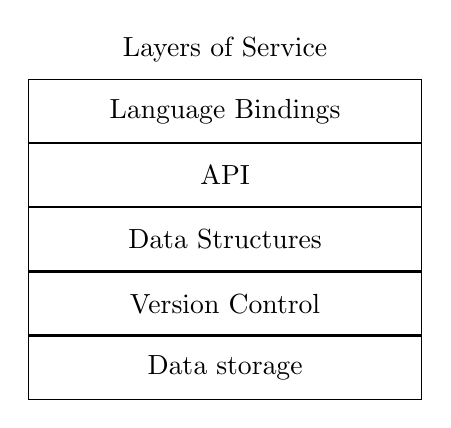
\begin{tikzpicture}

    \tikzstyle{thickarrow}=[line width=1mm,-triangle 45,postaction={draw, line width=3mm, shorten >=4mm, -}]
    \tikzstyle{hl}=[color=accentcolor]
    \tikzstyle{nn}=[circle, fill, style={fill=accentcolor,text=white}]
    \tikzstyle{s}=[draw, rectangle, minimum width = 5cm, minimum height=0.8cm]

    \begin{scope}[>=stealth']

      \node (langBinding) at (0,0)[s]{Language Bindings};
      \node (layers) [above=0.1cm of langBinding]{Layers of Service};
      \node (api) [below=0cm of langBinding,s]{API};
      \node (ds)[below=0cm of api,s]{Data Structures};
      \node (versionControl)[below=0cm of ds,s]{Version Control};
      \node (database)[below=0cm of versionControl,s]{Data storage};

    \end{scope}
    \end{tikzpicture}
    \end{figure}
  \end{center}
\end{frame}
\begin{frame}[fragile]
  \frametitle{EXAMPLE}
  \begin{center}
    \url{http://dsaas.pbit.co.za/workbench/graph/pierre/SimpleFriendsGraph/}
  \end{center}
\end{frame}

\section{Background}
% Background
\begin{frame}[fragile]
    \frametitle{version control}
\begin{center}
    \normalsize
    Ephemeral vs Persistent Data Structures


    
    \note{To provide version control capabilities on data, we first delve into the theory of persistent data structures.
    A data structure that does NOT provide access to its history is called an ephemeral data structure.
    All changes to an ephemeral data structure occur in-place and only the most recent version is ever available.
    An example of an ephemeral data structure are those found in the Java Collections Framework.
    (Add an image here??)
    
    On the other hand, a persistent data structure provides access to different versions of a similar---in the sense of expected operations---ephemeral data structure.
    The data structure starts at an initial version, and any subsequent updates creates new versions of the data structure.}


    \pause

    Types of persistence:

    \begin{tabular}{l  l}
        \pause
        \textbf{Partial Persistence} &
        \adjustbox{margin=0.1cm}{
          \resizebox{0.35\linewidth}{!}{
              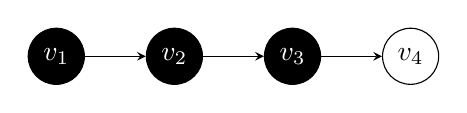
\begin{tikzpicture}[baseline={([yshift=-14pt]current bounding box.north)}]
              \begin{scope}[>=stealth]
                \node (v1) at (0,0) [circle,draw,style={fill=black, text=white}]{$v_1$};
                \node (v2) at (1.5,0) [circle,draw,style={fill=black, text=white}]{$v_2$};
                \node (v3) at (3,0) [circle,draw,style={fill=black, text=white}]{$v_3$};
                \node (v4) at (4.5,0) [circle,draw]{$v_4$};

                \draw[->] (v1) -- (v2);
                \draw[->] (v2) -- (v3);
                \draw[->] (v3) -- (v4);

              \end{scope}
              \end{tikzpicture}
          }
        }

        \\
        % \hline

        \pause
        \normalsize \textbf{Full Persistence} &
        \adjustbox{margin=0.1cm}{
          \resizebox{0.35\linewidth}{!}{
          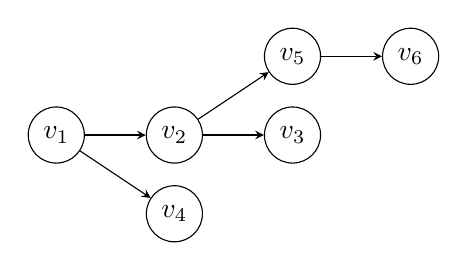
\begin{tikzpicture}[baseline={([yshift=-42pt]current bounding box.north)}]
          \begin{scope}[>=stealth]
            \node (v1) at (0,0) [circle,draw]{$v_1$};
            \node (v2) at (1.5,0) [circle,draw]{$v_2$};
            \node (v3) at (3,0) [circle,draw]{$v_3$};
            \node (v4) at (1.5,-1) [circle,draw]{$v_4$};
            \node (v5) at (3,1) [circle,draw]{$v_5$};
            \node (v6) at (4.5,1) [circle,draw]{$v_6$};

            \draw[->] (v1) -- (v2);
            \draw[->] (v1) -- (v4);
            \draw[->] (v2) -- (v3);
            \draw[->] (v2) -- (v5);
            \draw[->] (v5) -- (v6);

          \end{scope}
          \end{tikzpicture}
          }
        } \\

        % \hline
        \pause
        \normalsize \textbf{Confluent Persistence} &
        \adjustbox{margin=0.1cm}{
        \resizebox{0.35\linewidth}{!}{
        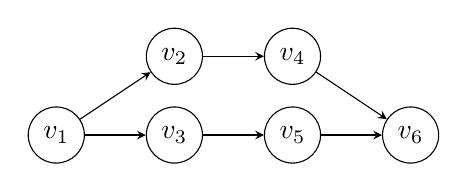
\begin{tikzpicture}[baseline={([yshift=-26pt]current bounding box.north)}]
        \begin{scope}[>=stealth]

          \node (v1) at (0,0) [circle,draw]{$v_1$};
          \node (v2) at (1.5,1) [circle,draw]{$v_2$};
          \node (v3) at (1.5,0) [circle,draw]{$v_3$};
          \node (v4) at (3,1) [circle,draw]{$v_4$};
          \node (v5) at (3,0) [circle,draw]{$v_5$};
          \node (v6) at (4.5,0) [circle,draw]{$v_6$};

          \draw[->] (v1) -- (v2);
          \draw[->] (v1) -- (v3);
          \draw[->] (v2) -- (v4);
          \draw[->] (v3) -- (v5);
          \draw[->] (v5) -- (v6);
          \draw[->] (v4) -- (v6);

        \end{scope}
        \end{tikzpicture}
        }}
    \end{tabular}
\end{center}

\end{frame}
\begin{frame}{path-copying}
	\centering
	Achieve full persistence using a technique called \emph{path-copying}
	% ~\cite{driscoll1986making}

	\begin{figure}
		\centering
		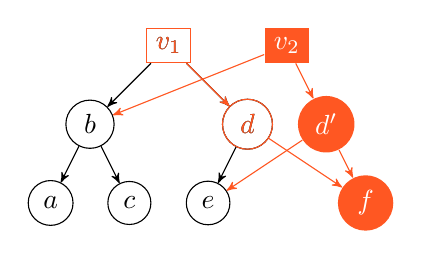
\begin{tikzpicture}

		\tikzstyle{thickarrow}=[line width=1mm,-triangle 45,postaction={draw, line width=3mm, shorten >=4mm, -}]
		\tikzstyle{hl}=[color=accentcolor]
		\tikzstyle{nn}=[circle, fill, style={fill=accentcolor,text=white}]
		\tikzstyle{nr}=[rectangle, fill, style={fill=accentcolor,text=white}]
		\tikzstyle{ns}=[nn, style={fill=grey}]

		\begin{scope}[>=stealth']


		\node (a2) at (1,-1) [circle,draw]{$b$};
		\node (b2) at (1.5,-2) [circle,draw]{$c$};
		\node (d2) at (0.5, -2) [circle,draw]{$a$};
		\node<1,2->(r2) at (2,0) [rectangle,draw]{$v_{1}$};
		\node<1,2->(c2) at (3,-1) [circle,draw]{$d$};
		\node(e2) at (2.5, -2) [circle,draw]{$e$};

		\node<2>(r2) at (2,0) [rectangle,draw, hl]{$v_{1}$};
		\node<2>(c2) at (3,-1) [circle,draw, hl]{$d$};

		\draw[->] (r2) -- (a2);
		\draw[->] (a2) -- (b2);
		\draw[->] (a2) -- (d2);
		\draw[->] (c2) -- (e2);

		\draw<1,2->[->] (r2) -- (c2);
		\draw<2>[->,hl] (r2) -- (c2);

		\visible<2->{\node(f) at (4.5, -2) [nn]{$f$};}
		\draw<2>[->, hl] (c2) -- (f);

		\visible<3->{\node(c3) at (4, -1) [nn]{$d'$};}
		\draw<3->[->, hl] (c3) -- (f);
		\draw<3->[->, hl] (c3) -- (e2);
		% \draw<3>[->, hl] (r2) -- (c3);

		\visible<3->{\node(r3) at (3.5, 0) [nr]{$v_{2}$};}
		\draw<3->[->, hl] (r3) -- (c3);
		\draw<3->[->, hl] (r3) -- (a2);

		\end{scope}
		\end{tikzpicture}
		\end{figure}
\end{frame}
% Quick reference to Requirements

\section{Development}
% Discuss design and implementation
\begin{frame}[fragile]
	\frametitle{Architecture Overview}

\newcommand{\staticServer}[0]{
	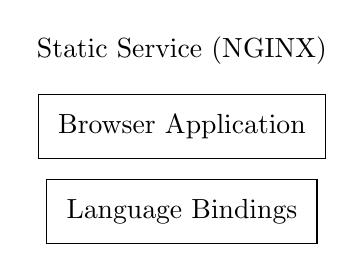
\begin{tikzpicture}

	\tikzstyle{stdrect}=[draw, rectangle, inner sep = 0.25cm];
    \begin{scope}[>=stealth]

    	\node (nginx) at (0,0) []{Static Service (NGINX)};
    	\node (browser) [below = 0.25cm of nginx, stdrect]{Browser Application};
    	\node (lang_binding) [below = 0.25cm of browser, stdrect]{Language Bindings};

    \end{scope}
    \end{tikzpicture}
}

\newcommand{\TPuser}[0]{
	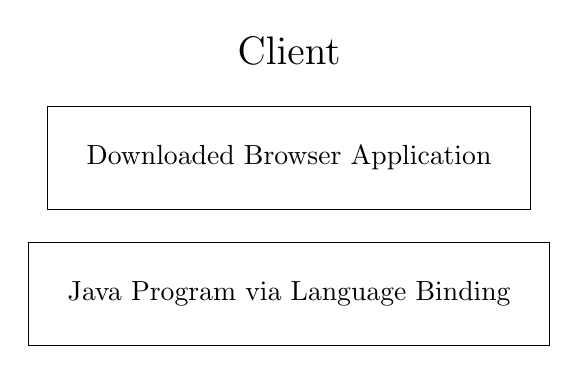
\begin{tikzpicture}

	\tikzstyle{stdrect}=[draw, rectangle, inner sep = 0.5cm, minimum width = 6cm];
    \begin{scope}[>=stealth]

    	\node (user_s) at (0,0) []{\Large Client};
    	\node (browser_screen) [below = 0.4cm of user_s, stdrect]{Downloaded Browser Application};
    	\node (lang_bindings_screen) [below = 0.4cm of browser_screen, stdrect]{Java Program via Language Binding};

    \end{scope}
    \end{tikzpicture}
}

\centering
\begin{tikzpicture}
	\begin{scope}[>=stealth]
		\node (center) at (0,0){};
		\node (leUser) [left = of center, draw, rectangle] {\resizebox{0.25\linewidth}{!}{\TPuser}};

    \node (dsaas) [right = 1.5cm of center]{};
    \node (static_server) [above right = -0.2cm and 0cm of dsaas, draw, rectangle] {\resizebox{0.2\linewidth}{!}{\staticServer}};
		\draw[->] (static_server) -- ++(-4,0) -- (leUser);
    \node (downloads) [above left = -0.8cm and 0.6cm of static_server] {HTTP};

    \pause

    \node (api_service) [below right = 0.2cm and -1.9cm of dsaas] {\resizebox{0.7\linewidth}{!}{\architectureOverview}};
    \node (as_coor) [above left = -0.8cm and -2.6cm of api_service, minimum width = 0.4cm]{};
    \draw[->] (as_coor) -- ++(-3,0) -- (leUser);
    \draw[<-] (as_coor) -- ++(-3,0) -- (leUser);

    \node (http) [below = 1.3cm of downloads] {HTTP};
    \node (web_sockets) [below = 0.05cm of http] {Web-Sockets};
	\end{scope}
\end{tikzpicture}
\end{frame}
\begin{frame}[fragile]
	\frametitle{Browser Application}
	\centering
		\begin{tabular}{c c}
		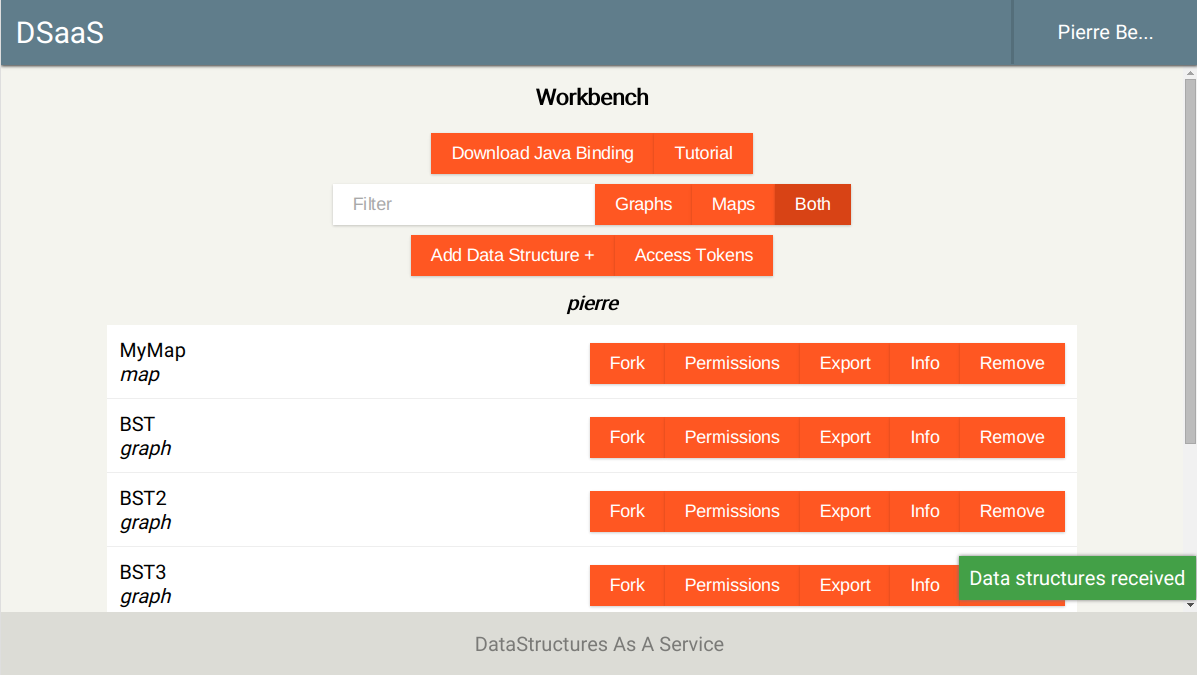
\includegraphics[width=0.47\textwidth]{images/workspace.png} &
		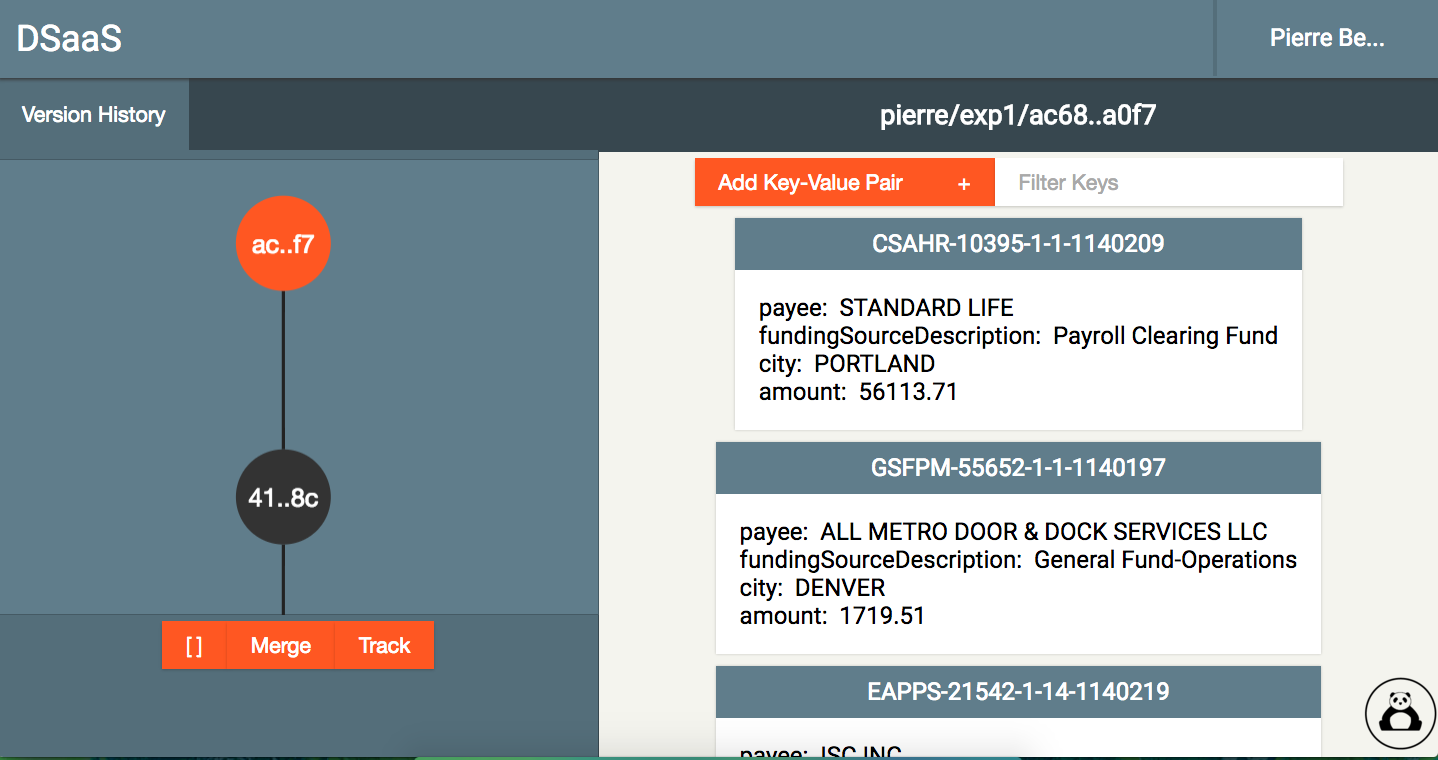
\includegraphics[width=0.47\textwidth]{images/map.png} \\
		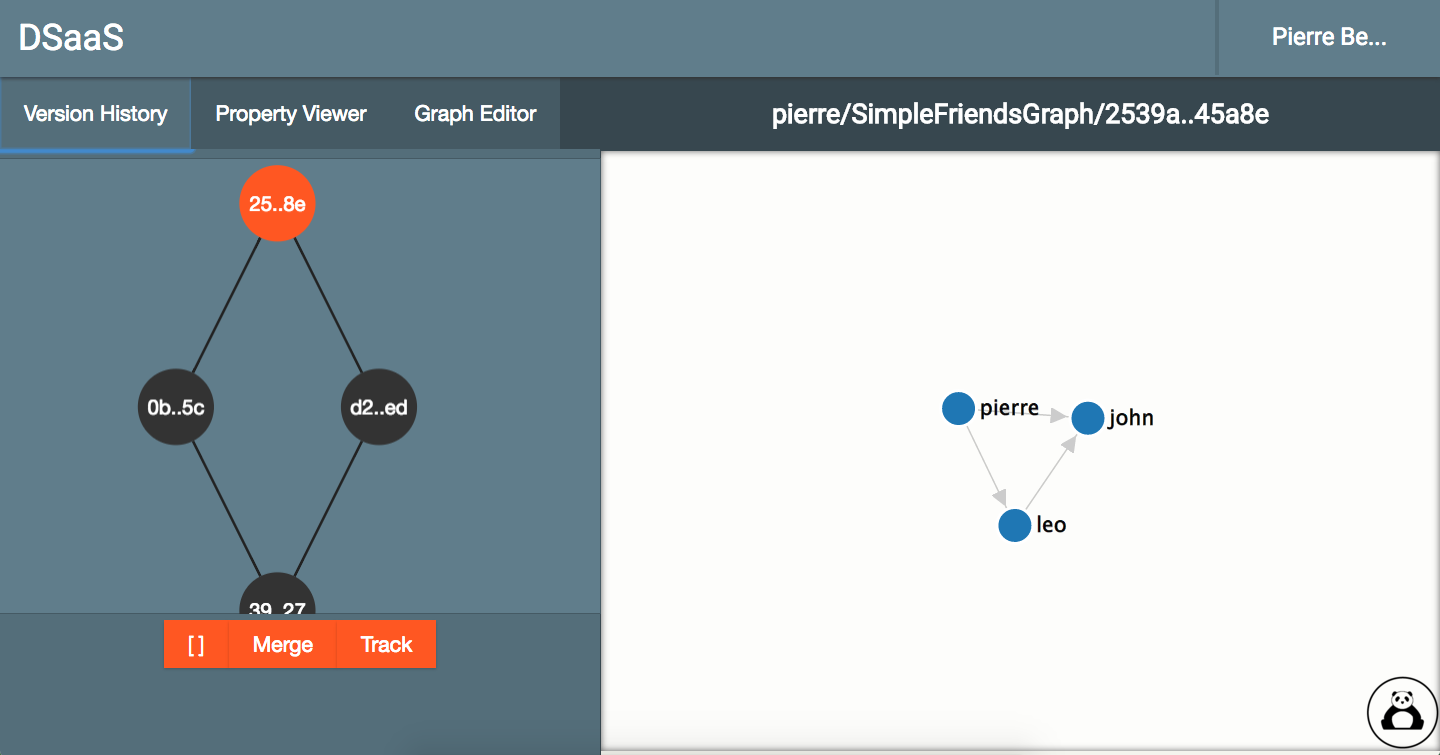
\includegraphics[width=0.47\textwidth]{images/graph.png} &
		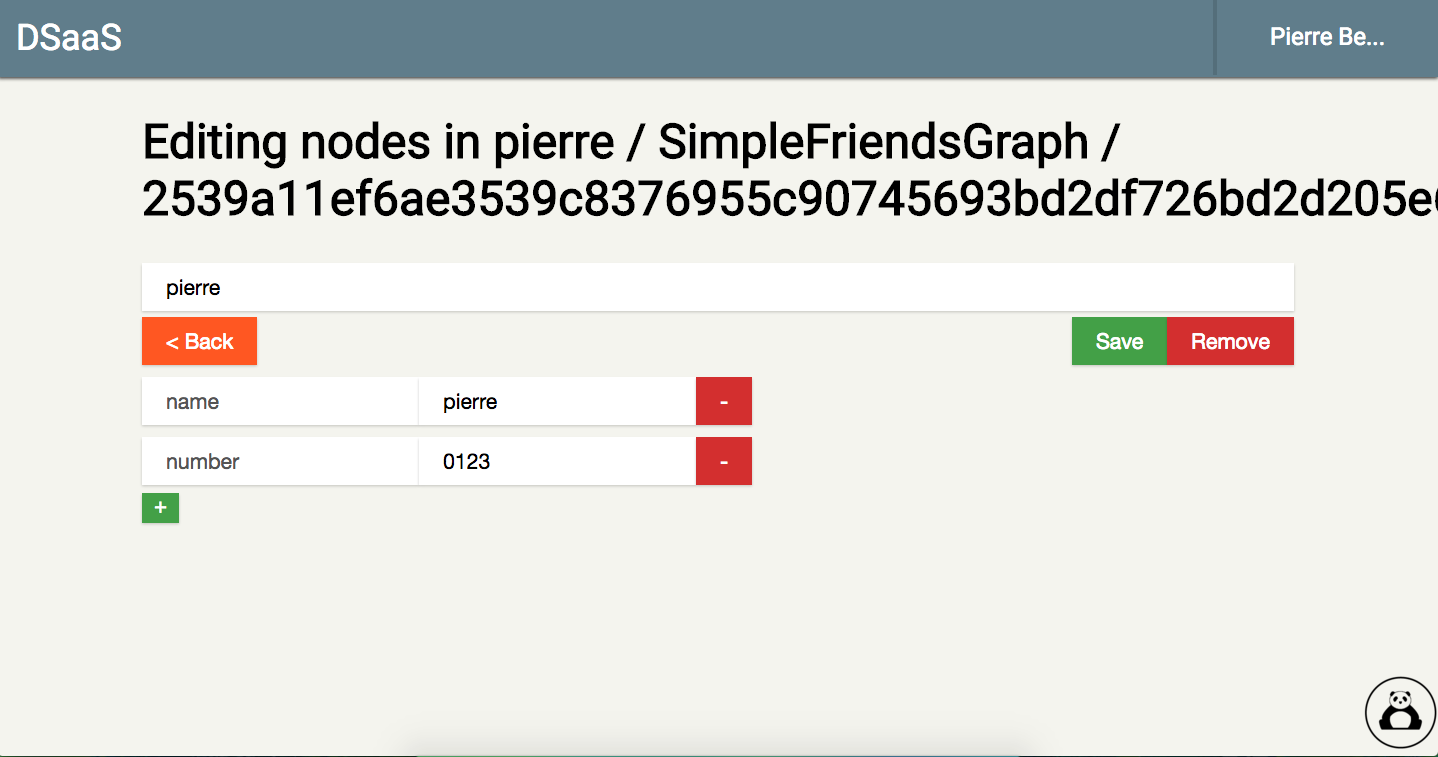
\includegraphics[width=0.47\textwidth]{images/edit.png}
	\end{tabular}
\end{frame}
% \begin{frame}[fragile]
	\frametitle{Adapted Flux Architecture}
	\note{The browser application uses an adapted Flux architecture, and ReactJS for rendering the HTML views.
	The Flux architecture is very straightforward, the idea is to have different units, where each unit receive information, processes the information and passes it on to the next one.
	Therefore it is a one-way data-flow of information and very easy to debug once things go wrong.}

\centering
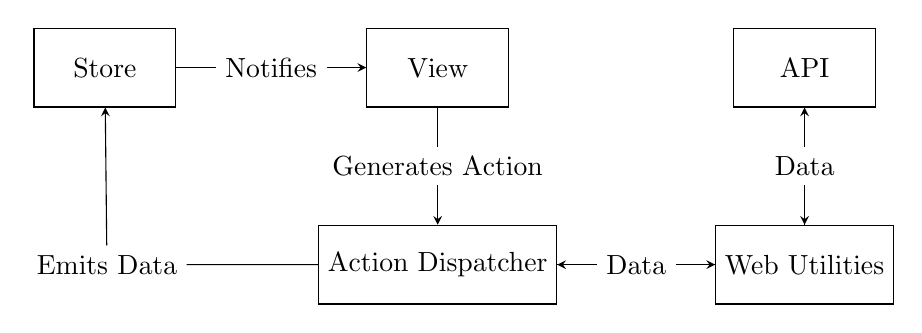
\begin{tikzpicture}
\tikzstyle{obj}=[draw, rectangle, minimum height=1cm, minimum width=1.8cm];
\begin{scope}[>=stealth]
  \node (dispatcher) at (-3.2,-2) {Emits Data};
  \node (action) at (1,-2) [obj]{Action Dispatcher};
  \node (generate) [above=0.5cm of action]{Generates Action};
  \node (views) [above=0.5cm of generate, obj]{View};
  \node (inform) [left=0.5cm of views]{Notifies};
  \node (stores) [left=0.5cm of inform, obj]{Store};
  \node (data) [right=0.5cm of action]{Data};
  \node (webutils) [right=0.5cm of data, obj]{Web Utilities};
  \node (data2) [above=0.5cm of webutils]{Data};
  \node (api) [above=0.5cm of data2, obj]{API};

  \draw[->] (action) -- (dispatcher) -- (stores);
  \draw (stores) -- (inform);
  \draw[->] (inform) -- (views);
  \draw (views) -- (generate);
  \draw[->] (generate) -- (action);
  \draw[->] (webutils) -- (data) -- (action);
  \draw[->] (action) -- (data) -- (webutils);
  \draw[->] (api) -- (data2) -- (webutils);
  \draw[->] (webutils) -- (data2) -- (api);
\end{scope}
\end{tikzpicture}

\end{frame}
% \begin{frame}[fragile]
	\frametitle{Language Bindings}
	\begin{center}
		\begin{tikzpicture}
			\node(java) at (0,0) {
\includegraphics[width=0.5\textwidth]{images/java.jpg}};
		\end{tikzpicture}
	\end{center}
\end{frame}
\begin{frame}[fragile]
	\frametitle{Back End}
	 \newcommand{\backEnd}[0] {
      \begin{tikzpicture}

      \tikzstyle{obj}=[draw, rectangle, minimum height=1cm, minimum width=2.2cm];
      \tikzstyle{bigobj}=[draw, rectangle, minimum height=2.5cm, minimum width=3.5cm];
      \tikzstyle{db}=[cylinder, shape border rotate=90, draw,minimum height=2cm,minimum width=2.6cm];

      \begin{scope}[>=stealth]
        \node (serverContainer) at (0,0) [draw, rectangle, minimum height=6.5cm, minimum width=7.2cm]{};
        \node (apiService) [above=-0.7cm of serverContainer]{API Service (NodeJS)};
        \node (nodejs) [above=0cm of apiService]{
\includegraphics[width=0.3\textwidth]{images/nodejs.png}};


        \node (db1) [right=0.4cm of serverContainer, db]{};
        \node (db1description) [above=-1cm of db1]{Key-Value};
        \node (db1description2) [below=0cm of db1description]{Database};
        \node (db1logo) [above=0cm of db1]{
\includegraphics[width=0.2\textwidth]{images/leveldb.png}};

        \node (db2) [left=0.4cm of serverContainer, db]{};
        \node (db2description) [above=-1cm of db2]{Document};
        \node (db2description2) [below=0cm of db2description]{Database};
        \node (db2logo) [above=0cm of db2]{
\includegraphics[width=0.2\textwidth]{images/mongodb.png}};


        \node (c) [above=-3.6cm of serverContainer]{};
        \node (apiContainer) [above left = -2.73cm and 0.65cm of c, draw, rectangle, minimum height=5.4cm, minimum width=2.6cm]{};
        \node [above=-0.5cm of apiContainer]{API Module};

        \node (general) [above=-1.6cm of apiContainer, obj]{General};
        \node (user) [below=0.2cm of general, obj]{User};
        \node (map) [below=0.2cm of user, obj]{Map};
        \node (graph) [below=0.2cm of map, obj]{Graph};

        \node (c2) [above=-4cm of serverContainer]{};
        \node (dsmodule) [right=-0.6cm of c2, draw, rectangle, minimum height=4.4cm, minimum width=3.8cm]{};
        \node [above=-0.5cm of dsmodule]{Data Structure Module};

        \node (dagstore) [above=-1.6cm of dsmodule, obj]{Version History};
        \node (vtstore) [below=0.32cm of dagstore, obj]{Versioned Trie};
        \node (graphstore) [below=0.32cm of vtstore, obj]{Versioned Graph};


        \draw [->] (general) -- (db2);
        \draw [->] (general) -- (dsmodule);
        \draw [->] (user) -- (db2);
        \draw [->] (map) -- (db2);
        \draw [->] (graph) -- (db2);
        \draw [->] (db2) -- (general);
        \draw [->] (db2) -- (user);
        \draw [->] (db2) -- (map);
        \draw [->] (db2) -- (graph);

        \draw[->] (dagstore) -- (db1);
        \draw[->] (vtstore) -- (db1);
        \draw[->] (db1) -- (vtstore);
        \draw[->] (db1) -- (dagstore);
        \draw[->] (vtstore) -- (dagstore);
        \draw[->] (graphstore) -- (vtstore);
        \draw[->] (map) -- (vtstore);
        \draw[->] (graph) -- (graphstore);

      \end{scope}
     \end{tikzpicture}
   }

   \centering
   \begin{tikzpicture}
    \node (api_service) at (0,0) {\resizebox{\linewidth}{!}{\backEnd}};
   \end{tikzpicture}
\end{frame}
\begin{frame}[fragile]
	\frametitle{Versioned Trie}

	\begin{itemize}
		\item Based on the Hashed Array Mapped Trie (HAMT).
		\item Implemented on storage instead of in memory.
		\item Three-Way Merge operation for confluent persistence.
		\item Detecting transpositions through Zobrist hashing.
	\end{itemize}

\end{frame}
\begin{frame}[fragile]
	\frametitle{Hashed Array Mapped Trie (HAMT)}

	\newcommand{\hl}[2]{\color<#1>{accentcolor}#2\color{primary}}

	% \begin{minipage}{0.5\textwidth}
	% 	Insert keys: \texttt{A}, \texttt{B}, \texttt{C} and \texttt{D}.

	% 	Hash \texttt{A} = \ldots\ 00000 00000 \hl{2}{00010}

	% 	\onslide<3->{Hash \texttt{B} = \ldots\ 00000 \hl{7-9}{00001}\ \hl{3-6}{00001}}

	% 	\onslide<6->{Hash \texttt{C} = \ldots\ \hl{10}{00011}\ \hl{7-9}{00011}\ \hl{6}{00001}}

	% 	\onslide<10->{Hash \texttt{D} = \ldots\ \hl{10}{00000}\ 00011 00001}

	% \end{minipage}%
	% \begin{minipage}{0.5\textwidth}
	% 	% \begin{figure}
	% 	  \centering
	% 	    \begin{tikzpicture}

	% 	    \tikzstyle{obj}=[draw, rectangle, minimum height=0.5cm, minimum width=1.5cm];
	% 	    \tikzstyle{arr}=[draw, rectangle, minimum height=0.5cm, minimum width=0.5cm];
	% 	    \tikzstyle{bigobj}=[draw, rectangle, minimum height=2.5cm, minimum width=3.5cm];
	% 	    \tikzstyle{db}=[cylinder, shape border rotate=90, draw,minimum height=2cm,minimum width=2.6cm];
	% 	    \tikzstyle{bmp}=[arr, style={fill=gray,text=white}];

	% 	    \begin{scope}[>=stealth]
	% 			\node (level0) at (0,0) {};

	% 			\node<1>(level0_2) [left=0cm of level0, arr] {Array Of Pointers};
	% 			% \node (level0_4) [right=0cm of level0_2, arr] {};
	% 			\node<1>(bitmap0) [left=0cm of level0_2, bmp] {Bitmap};
	% 			% \node (ext_1) [right=0cm of level0_4]{\ldots};
	% 			\onslide<1>{\node (rootLabel) [above left=0cm and -0.48cm of level0_2] {Node};}
	% 			\node<1>(pointOfBitmap)[below=0cm of level0_2]{\begin{varwidth}{6cm}
	% 			The bitmap indicates the presence, and is used to determine the position, of a pointer within the pointer array.
	% 			\end{varwidth}};

	% 			\node<1>(pointOfArray)[below=0cm of pointOfBitmap]{\begin{varwidth}{6cm}
	% 			The array of pointers can point to another node or a key.
	% 			\end{varwidth}};

	% 			\pause

	% 			\node(level0_2) [left=0cm of level0, arr] {};
	% 			\node<2>(bitmap0) [left=0cm of level0_2, bmp] {};


	% 			\node (level0_2) [left=0cm of level0, arr] {$\cdot$};

	% 			\node<2>(bitmap0) [left=0cm of level0_2, bmp] {\ldots 0100};
	% 			\node<2-4>(package1) [below=0.5cm of level0_2]{A};
	% 			\draw<2-4>[->] (level0_2) -- (package1);

	% 			\onslide<2>{
	% 				\node (indicator) [above = 0.5cm of bitmap0] {
	% 					\begin{varwidth}{4cm}
	% 						\small 2nd bit set, indicating that there exists a pointer in the array with a hash suffix of 2.
	% 					\end{varwidth}};
	% 				\node (anchor) [above right = -0.2cm and -0.7cm of bitmap0]{};
	% 				\draw[->] (indicator) -- (anchor);
	% 			}

	% 			\pause

	% 			\node<3-4>(a) [right = 0cm of level0_2, arr]{$?$};
	% 			\node<3-4>(b) [left = 0cm of level0_2, arr]{$?$};
	% 			\node<3>(bitmap0) [left=0cm of b, bmp] {\ldots 0100};

	% 			\pause

	% 			\node<4>(bitmap0) [left=0cm of b, bmp] {\ldots 0110};

	% 			\pause

	% 			\node<5->(bitmap0) [left=0cm of level0_2, bmp] {\ldots 0110};
	% 			\node (level0_4) [right=0cm of level0_2, arr] {$\cdot$};

	% 			\node (package1) [right=0.5cm of level0_4]{A};
	% 			\draw[->] (level0_4) -- (package1);

	% 			\onslide<5-6>{
	% 				\node (package2) [below=0.5cm of level0_2]{B};
	% 				\draw[->] (level0_2) -- (package2);
	% 			}

	% 			\pause
	% 			\pause

	% 			\node<7> (bitmap1)[below= 0.5cm of level0_2, bmp] {\ldots 0000};
	% 			\draw<7>[->] (level0_2) -- (bitmap1);

	% 			\pause

	% 			\node<8> (bitmap1)[below= 0.5cm of level0_2, bmp] {\ldots 0010};
	% 			\draw<8>[->] (level0_2) -- (bitmap1);
	% 			\node<8>(level1_B) [right=0cm of bitmap1, arr] {$\cdot$};
	% 			\node<8>(package2) [below=0.5cm of level1_B]{B};
	% 			\draw<8>[->] (level1_B) -- (package2);

	% 			\pause

	% 			\node (bitmap1) [below= 0.5cm of level0_2, bmp] {\ldots 1010};
	% 			\draw[->] (level0_2) -- (bitmap1);
	% 			\node(level1_B) [right=0cm of bitmap1, arr] {$\cdot$};
	% 			\node (level1_C) [right=0cm of level1_B, arr] {$\cdot$};
	% 			\node(package2) [below=0.5cm of level1_B]{B};
	% 			\draw[->] (level1_B) -- (package2);
	% 			\onslide<9>{\node (package3) [below=0.5cm of level1_C]{C};}


	% 			\draw[->] (level0_4) -- (package1);

	% 			\onslide<9>{\draw[->] (level1_C) -- (package3);}

	% 			\pause

	% 			\node (bitmap2) [below right = 0.5cm and -0.2cm of level1_C, bmp] {\ldots 1001};
	% 			\node (level2_1) [right=0cm of bitmap2, arr] {$\cdot$};
	% 			\node (level2_2) [right=0cm of level2_1, arr] {$\cdot$};

	% 			\node (package3) [below=0.5cm of level2_2]{C};
	% 			\node (package4) [below=0.5cm of level2_1]{D};

	% 			\draw[->] (level2_2) -- (package3);
	% 			\draw[->] (level1_C) -- (bitmap2);
	% 			\draw[->] (level2_1) -- (package4);

	% 	    \end{scope}
	% 	    \end{tikzpicture}
	% 	  % \caption{An example of a typical HAMT, where the grey blocks are the bitmaps (indicating the presence of pointers), the white blocks are the array block cells filled with the label of the edge leading to next node or value, and the black dots are the values that this trie store.
	% 	  % The hashed keys of this trie are 2\ldots, 42\ldots and 4E1\ldots in hexadecimal (the rest of the key identifiers are irrelevant for this example trie). }
	% 	  % \label{fig:hamt-diagram}
	% 	% \end{figure}
	% \end{minipage}

	\begin{figure}
	  \centering
	    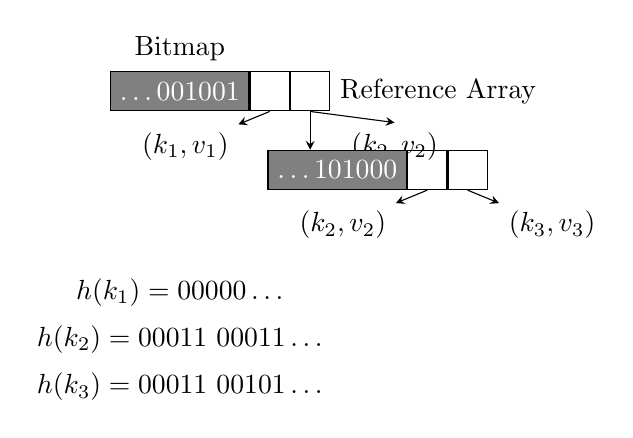
\begin{tikzpicture}

	    \tikzstyle{obj}=[draw, rectangle, minimum height=0.5cm, minimum width=1.5cm];
	    \tikzstyle{arr}=[draw, rectangle, minimum height=0.5cm, minimum width=0.5cm];
	    \tikzstyle{bigobj}=[draw, rectangle, minimum height=2.5cm, minimum width=3.5cm];
	    \tikzstyle{db}=[cylinder, shape border rotate=90, draw,minimum height=2cm,minimum width=2.6cm];
	    \tikzstyle{bmp}=[arr, style={fill=gray,text=white}];

	    \begin{scope}[>=stealth]
	      \node (level0) at (0,0) {};
	      \node (level0_2) [left=0cm of level0, arr] {};
	      \node (level0_4) [right=0cm of level0_2, arr] {};
	      \node<1-2>(bitmap0) [left=0cm of level0_2, bmp] {\ldots000000};

	      % \node (rootLabel) [above=0.5cm of level0_2] {Root Node};
	      \node (bitmapLabel)[above=0cm of bitmap0] {Bitmap};
	      \node (refArrayLabel) [right=0cm of level0_4]{Reference Array};

	      \pause

	      \node (hashkey1) [below=2cm of bitmap0 ]{$h(k_{1}) = 00000\ldots$};

	      \pause

	      \node<3>(bitmap0) [left=0cm of level0_2, bmp] {\ldots000001};

	      \node (package1) [below left=0.2cm of level0_2]{$(k_{1}, v_{1})$};
	      \draw[->] (level0_2.south) -- (package1);

	      \pause

	      \node (bitmap0) [left=0cm of level0_2, bmp] {\ldots001001};
	      \node<4>(package2) [below right=0.2cm of level0_4]{$(k_{2}, v_{2})$};
	      \draw<4>[->] (level0_4.south) -- (package2.north);
	      \node (hashkey2) [below=0cm of hashkey1]{$h(k_{2}) = 00011$ $00011\ldots$};

	      \pause

	      \node (hashkey3) [below=0cm of hashkey2]{$h(k_{3}) = 00011$ $00101\ldots$};


	      \node (level1) at (2, -1) {};
	      \node (level1_0) [left=0cm of level1, arr] {};
	      \node (level1_5) [right=0cm of level1_0, arr] {};
	      % \node<2>(bitmap1) [left=0cm of level1_0, bmp] {\ldots000000};
	      \node (bitmap1) [left=0cm of level1_0, bmp] {\ldots101000};

	      \draw[->] (level0_4) -- (level0_4 |- bitmap1.north);

	      \node (package2) [below left=0.2cm of level1_0]{$(k_{2}, v_{2})$};
	      \node (package3) [below right=0.2cm of level1_5]{$(k_{3}, v_{3})$};

	      \draw[->] (level1_0.south) -- (package2);
	      \draw[->] (level1_5.south) -- (package3);

	    \end{scope}
	    \end{tikzpicture}
	  \caption{An example of an HAMT\@. The grey blocks represent the bitmaps, and the white cells represent the array of references to key--value pairs stored in this trie.}
	  %, and the key--value pairs stored by this trie are \todo{represented as the alphabet characters}.}
	  \label{fig:hamt-diagram-path-copying}
	\end{figure}
\end{frame}
% \begin{frame}[fragile]
	\frametitle{Version History}
  An implementation of a graph recording the relationships between different versions.
  Used for navigation of the persistent data structures.

  \begin{center}
    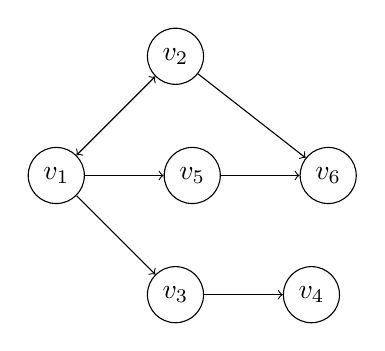
\begin{tikzpicture}
      \tikzstyle{obj}=[draw, circle];

      \node (v1) at (0,0)[obj]{$v_{1}$};
      \node (v2) [above right=of v1, obj]{$v_{2}$};
      \node (v3) [below right=of v1, obj]{$v_{3}$};
      \node (v4) [right=of v3, obj]{$v_{4}$};
      \node (v5) [right=of v1, obj]{$v_{5}$};
      \node (v6) [right=of v5, obj]{$v_{6}$};

      \draw [<->] (v1) -- (v2);
      \draw [->] (v1) -- (v3);
      \draw [->] (v1) -- (v5);

      \draw [->] (v2) -- (v6);
      \draw [->] (v5) -- (v6);

      \draw [->] (v3) -- (v4);

    \end{tikzpicture}
  \end{center}
\end{frame}

\section{Evaluation}
\begin{frame}[fragile]
	\frametitle{Evaluation}

	\begin{minipage}{0.5\textwidth}
		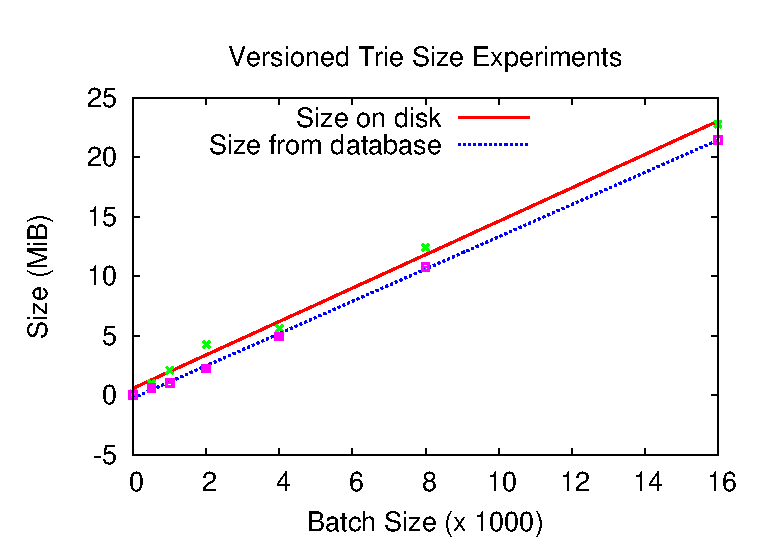
\includegraphics[width=\textwidth]{images/chart.eps}
	\end{minipage}%
	\begin{minipage}{0.5\textwidth}
		\begin{description}
			\item[Insertion:] 1 = adding 12 ephemeral data items
			\item[Removal:] 1 = adding 10 ephemeral data  items
			\item[Merging:] 16\,000 x 16\,000 elements = increase of 650 KiB ~ 6000 ephemeral items
		\end{description}
	\end{minipage}

\end{frame}
\begin{frame}[fragile]
\frametitle{Latency}
\begin{table}
  \begin{tabular}{l | l}
    Remote Server (Library Binding) & 206 \\
    Localhost (Library Binding) & 7.6 \\
    Core (JavaScript) & 2
  \end{tabular}
  \label{table:latency}
\end{table}
The latency (in ms) for the \emph{put} operation using the library binding to connect to a remote server and the localhost, and using JavaScript to test it on the core system.
\end{frame}
\begin{frame}[fragile]
	\frametitle{Compared to Dat}
  \begin{center}
  	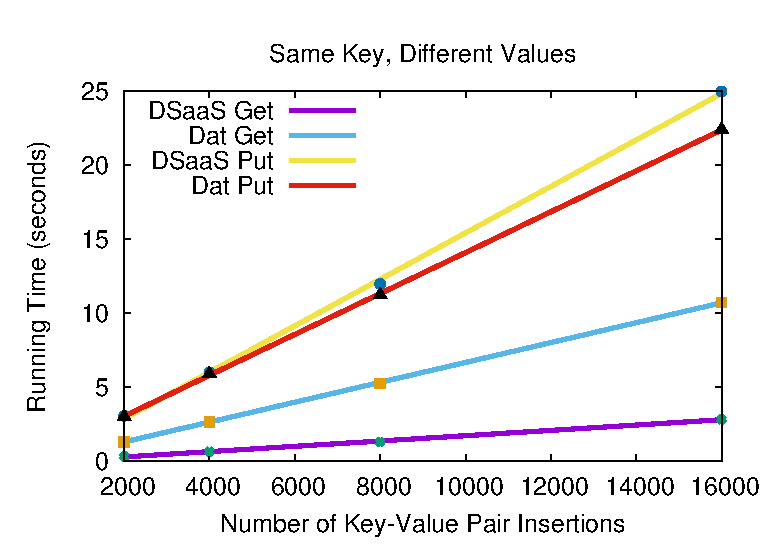
\includegraphics[width=0.5\textwidth]{images/same_key_diff_versions.eps}
  	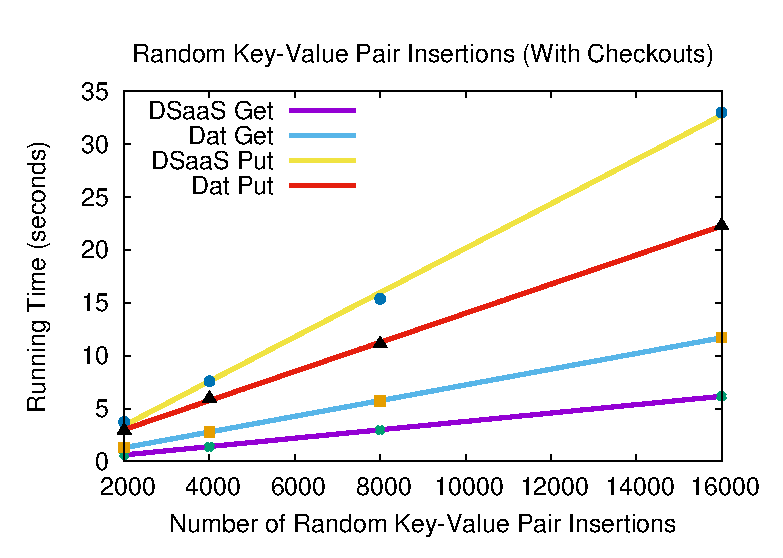
\includegraphics[width=0.5\textwidth]{images/kvpair.eps}
    \\
    Dat is available at \url{http://dat-data.com/}
  \end{center}
\end{frame}

\begin{frame}[fragile]
  \frametitle{Compared to Dat}
  \begin{center}
  	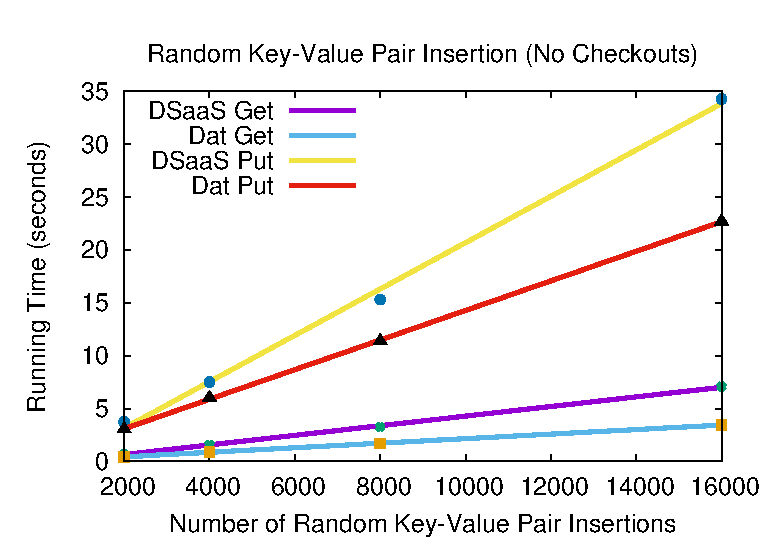
\includegraphics[width=0.5\textwidth]{images/samver.eps}
    \\
    Dat is available at \url{http://dat-data.com/}
  \end{center}
\end{frame}

\section{Conclusion}
% \begin{frame}{fragile}
	\frametitle{Features}

\begin{tikzpicture}
    \tikzstyle{obj}=[fill=accentcolor, draw=none, rectangle, minimum width=2.2cm,minimum height=0.8cm];
    \tikzstyle{sobj}=[obj, minimum width=1cm];
    \tikzstyle{link}=[color=accentcolor];
	\begin{scope}[>=stealth]
    
    
    \node(web_interface_image) at (0,0)[draw, circle, color=accentcolor]{
\includegraphics[width=0.0984\textwidth]{images/web-interface-3.png}};
    \node(web_interface_label) [above = 0cm of web_interface_image] {Browser Application};
     
		\pause
		
	    \node(access_control_image) [right = 1.6cm of web_interface_image, draw, circle, color=accentcolor]{
\includegraphics[width=0.08\textwidth]{images/access-control.jpg}};
	    \node(access_control_label) [above = 0cm of access_control_image] {Access Control};
    
	    \pause

		\node(data_types_image) [right = 1.6cm of access_control_image, draw, circle, color=accentcolor]{
\includegraphics[width=0.08\textwidth]{images/data-types.png}};
	    \node(data_types_label) [above = 0cm of data_types_image] {Multiple Data Types};


	    \pause

	    \node(language_binding_image) [right = 1.6cm of data_types_image, draw, circle, color=accentcolor]{
\includegraphics[width=0.1152\textwidth]{images/chain.png}};
	    \node(language_binding_label) [above = 0cm of language_binding_image] {Language Bindings};

    
		\pause

		\node(import_export_image) [below = of web_interface_image, draw, circle, color=accentcolor]{
\includegraphics[width=0.08\textwidth]{images/import-export.png}};
	    \node(import_export_label) [above = 0cm of import_export_image] {Import and Export};
	    
	    \pause

	    \node(fork_image) [right = 1.6cm of import_export_image, draw, circle, color=accentcolor]{
\includegraphics[width=0.08\textwidth]{images/fork.png}};
	    \node(fork_label) [above = 0cm of fork_image] {Fork};

		\pause

	   \node(merge_image) [right = 1.6cm of fork_image, draw, circle, color=accentcolor]{
\includegraphics[width=0.08\textwidth]{images/merge.png}};
	   \node(merge_label) [above = 0cm of merge_image] {Merge};

	   \pause

	   \node(diff_image) [right = 1.6cm of merge_image, draw, circle, color=accentcolor]{
\includegraphics[width=0.08\textwidth]{images/diff.png}};
	    \node(diff_label) [above = 0cm of diff_image] {Difference};
	    
    \end{scope}
\end{tikzpicture}


\end{frame}
\input{conclusion}

\printbibliography

\begin{frame}
\centering\Huge
	Questions? \\
	
\includegraphics[width=0.4\textwidth]{images/panda_logo.png}
\end{frame}

\end{document}
